

\chapter{مفاهیم اولیه}

دومین فصل این پایان‌نامه به معرفی مفاهیمی می‌پردازد که در پایان‌نامه مورد استفاده قرار می‌گیرند.


%----------------------------- مقدمه ----------------------------------


\section{ترواهای سخت‌افزاری}
تروا‌های سخت‌افزاری مدارهایی با عملیات بداندیشانه هستند که ممکن است به مدار اصلی افزوده شوند. این تروا‌ها در مراحل مختلف از زمان طراحی در سطح انتقال ثبات RTL\footnote{\lr{Register Transfer Level}} تا ساخت تراشه ممکن است توسط افراد یا شرکتها و کارخانجات غیرمطمئن در مدار جاسازی شوند
$\cite{tehranipoor2010survey}$. 
فرآیند طراحی و ساخت مدارات مجتمع شامل چهار مرحله عمده است: طراحی سطح انتقال ثبات(شامل مشخصه مدار، بلاکهای IP\footnote{\lr{Intellectual Property}} و افراد طراح)، طراحی فیزیکی(شامل ابزارهای CAD\footnote{\lr{Computer Aided Design}} مدل‌ها و افراد طراح)، ساخت(شامل تولید ماسکها و لیتوگرافی)، و آزمون ساخت(شامل آزمودن ویفر و بسته بندی). در فرآیند طراحی در سطح RTL و فیزیکی فرض می‌شود که ابزارهای CAD مطمئن و قابل اعتماد هستند چرا که توسط شرکتهای معتبر طراحی می‌شوند. اما بلاکهای  IP مدل‌ها و سلول‌های استانداردی که توسط طراحان استفاده می‌شوند می‌توانند نامطمئن باشند. همچنین فاز ساخت نیز می‌تواند نامطمئن باشد.

این تروا‌های سخت‌افزاری می‌توانند تراشه‌ها را تخریب کنند، باعث رفتار اشتباه شوند یا دسترسی حمله‌کننده‌ها به کلیدهای سرّی را فراهم کنند. از سال 2007 محققین برای یافتن روش‌های تشخیص تروا برای جلوگیری از آسیب‌های آن، پژوهش‌هایی انجام داده‌اند $\cite{agrawal2007trojan}$. روش عمومی این است که با اعمال تعداد زیادی ورودی مختلف، تروا را فعال کنند و با مشاهده تفاوت در رفتار مدار بدون تروا با مدار دارای تروا، حضور تروا را تشخیص دهند. با این وجود، فعال‌سازی اغلب تروا‌ها کار بسیار مشکلی است. از طرفی ارزیابی کامل تمام بخش‌های مداری که شامل میلیون‌ها گیت است، زمان بسیار زیادی لازم دارد. یکی از راههای جایگزین استفاده از اطلاعات پارامترهای جانبی مدار از قبیل توان مصرفی، تاخیر مسیرها و جریان نشتی است. مدارات حاوی تروا پارامترهای جانبی متفاوتی با مدارات بدون تروا دارند. مشکل اصلی این روش‌ها این است که اثر تروا بر پارامترهای جانبی ممکن است توسط اثر تغییرات فرآیند پوشش داده شود. از طرفی تشخیص تروا‌های داخل IP‌ در این روش بسیار مشکل است چرا که اکثر IP ‌ها‌‌ به صورت کد RTL ارائه می‌شوند.

به علت معایبی که روش‌های موجود دارند، لازم است روش‌های جدیدی ارائه شود تا امنیت و قابلیت اطمینان سیستم‌های الکترونیکی، بخصوص سیستم‌های با کاربرد بحرانی را بالا ببرد. یکی از اهداف ما در این پژوهش ارائه روش‌هایی برای تشخیص تروا‌های سخت‌افزاری به طور موثر است. هدف دیگر ما ارائه راهکارهایی برای مقاوم سازی مدار در برابر تروا است. در هر دو بخش ایده اصلی این است که به نحوی کنترل‌پذیری و مشاهده‌پذیری نقاط مختلف مدار را افزایش دهیم. چرا که اغلب طراحان تروا، تروا‌ها را در نقاطی درج می‌کنند که با اعمال بردارهای آزمون نتوان به راحتی به ورودی‌های فعالساز آنها  و خروجی‌های آنها دسترسی داشت. بنابراین نمی‌توان آنها را به راحتی فعال نمود و اثرشان را در خروجی یا پارامترهای جانبی مشاهده کرد.


\section{دسته‌بندی تروا‌های سخت‌افزاری}

برای تسهیل فرآیند تشخیص تروا یا کاهش اثرات مخرب آن و ابداع روش‌های محافظت در برابر تروا، لازم است تا ابتدا تروا‌های سخت‌افزاری دسته‌بندی شوند و براساس این دسته‌بندی کارهای بعدی انجام شود. پژوهش‌های بسیاری در این زمینه انجام شده‌است
$\cite{tehranipoor2010survey,wolff2008towards,wang2008detecting,karri2010trustworthy,rad2008power}$.
تروا‌های سخت‌افزاری را می‌توان براساس پنج ویژگی دسته‌بندی نمود: 

\begin{itemize}
	\item فازی از طراحی که تروا در آن به مدار افزوده می‌شود
	\item سطح انتزاع
	\item روش فعال شدن تروا
	\item عملکرد تروا
	\item محل قرارگیری
\end{itemize}

در ادامه به بررسی این ویژگی‌ها می‌پردازیم.

\subsection{فاز درج تروا}
\subsubsection{الف) فاز مشخصات}
در این فاز مشخصات سیستم(هدف، محیط عملکرد، عملیات مورد انتظار، اندازه، توان، تاخیر و ...) تعریف می‌شود. در این فاز می‌توان مشخصه عملیاتی یا سایر قیود طراحی را تغییر داد. تروا در این فاز ممکن است نیازمندی‌های زمانی سخت‌افزار را دست کاری کند.
\subsubsection {ب) فاز طراحی}
در فاز طراحی قیود عملیاتی،  منطقی، زمانبندی و فیزیکی برای نگاشت طرح روی تکنولوژی مقصد مدنظر قرار می گیرد. در این فاز طراحان ممکن است از بلاکهای IP دیگران یا سلولهای استاندارد آنها استفاده کنند که ممکن است شامل تروا باشند. 
\subsubsection {ج) فاز ساخت}
در این فاز مجموعه ماسکها ساخته می‌شود و ویفرها براساس این ماسکها تولید می‌شوند. تغییر ماهرانه ماسکها می‌تواند منجر به اثرات مخربی شود یا تغییر ترکیبات شیمیایی در طی فرآیند تولید می‌تواند منجر به افزایش پدیده مهاجرت الکترونی در مدارات بحرانی شود و فرآیند خراب شدن مدار را تسریع کند.
\subsubsection {د) فاز مونتاژ}
در فاز مونتاژ تراشه و سایر عناصر سخت‌افزاری روی PCB  مونتاژ می‌شوند. هر واسطی که دو عنصر را به هم مرتبط کند، پتانسیل درج تروا را دارد. برای مثال سیم بدون روکشی که روی PCB به یک عنصر وصل شده‌است، تزویج الکترومغناطیس  بین سیگنال‌های روی بورد و سیگنال‌های محیط را باعث می‌شود. از این مساله می‌توان برای نشت اطلاعات یا تزریق اشکال استفاده کرد.

\subsubsection {ه) فاز آزمون}
در این فاز امکان درج تروا نیست ولی اهمیت آن به خاطر شانس تشخیص تروا است. اگر خود فرآیند آزمون قابل اعتماد باشد، می‌توان از آن برای تشخیص تروا استفاده کرد.


\subsection{سطح انتزاع}
\subsubsection {الف) سطح سیستم}
در سطح سیستم عناصر سخت‌افزاری متفاوت، اتصالات، و پروتکل‌های ارتباطی که استفاده می‌شوند، توصیف می‌شوند. در این سطح تروا ممکن است توسط عناصر داخل سخت‌افزار هدف فعال شود. برای مثال ممکن است مقادیر کد ASCII که از صفحه کلید گرفته می‌شود، باعث فعال شدن تروا شود.
\subsubsection {ب) سطح انتقال ثبات}
در این سطح هر ماژول عملیاتی برحسب ثبات‌ها، سیگنال‌ها و عملیات بولی توصیف می‌شود. از آنجا که در این سطح حمله‌کننده کنترل کامل بر عملیات سخت‌افزاری دارد، تروا به راحتی قابل طراحی و درج است. برای مثال یک تروا ممکن است تعداد دفعات اجرای مرحله‌ای از الگوریتم رمز نگاری را با دو برابر کردن گام حلقه تکرار، نصف کند و منجر به اشکال در سیستم رمزنگاری شود.
\subsubsection {ج) سطح دروازه‌های منطقی}
در این سطح، طراحی به صورت اتصال بین دروازه‌های منطقی توصیف می‌شود. در این مرحله حمله‌کننده به سیستم به راحتی می‌تواند جنبه‌های مختلف تروای که می خواهد درج کند(مانند اندازه و محل درج) را کنترل کند.  در این سطح تروا می‌تواند یک مقایسه‌گر ساده با دروازه‌های منطقی XOR باشد که بر سیگنال‌های داخلی تراشه نظارت می‌کند. تروا می‌تواند ترکیبی یا ترتیبی باشد. این تروا‌ها معمولا برای تغییر عملکرد طرح به کار می روند و از این رو به تروا‌های عملیاتی معروفند.
\subsubsection {د) سطح ترانزیستور}
در این سطح، مدار با استفاده از  ترانزیستورهایی که برای ساختن دروازه‌های منطقی استفاده می‌شوند، توصیف می‌شود. در این سطح، طراح تروا کنترل کاملی بر مشخصه‌های مداری سیستم مانند توان و زمانبندی دارد. تروا ممکن است با افزودن یا کاستن ترانزیستورها یا تغییر اندازه آنها برای تغییر پارامترهای مدار، درج شده باشند. تروا‌های این سطح نیز از جمله تروا‌های عملیاتی هستند.
\subsubsection {ه)سطح layout}
در این سطح ابعاد و محل همه عناصر مدار توصیف می‌شود. در این سطح تروا ممکن است از طریق تغییر اندازه سیم‌ها، فواصل بین عناصر مدار و تخصیص دوباره لایه‌های فلز درج شود. برای مثال تغییر عرض سیم‌های فلزی شبکه ساعت در تراشه می‌تواند منجر به انحراف سیگنال ساعت شود. به این تروا‌ها تروا‌های پارامتری می گویند. 
بسته به تعداد دروازه‌های منطقی که توسط تروا در مدار درج می‌شود، تروا می‌تواند به دو دسته کوچک و بزرگ دسته‌بندی شود. همچنین براساس توزیع آن در طرح، به دو دسته متمرکز و توزیع شده دسته‌بندی شود.

\subsection{روش فعال شدن تروا}
بعضی از تروا‌ها به نحوی طراحی می‌شوند که همیشه فعال هستند. بعضی دیگر، تا زمانی که توسط سیگنال یا الگوی خاصی تحریک نشوند، فعال نمی‌شوند.  معمولاً تروا‌های پارامتری از دسته «همیشه فعال» هستند. تروا‌هایی که تحریک می‌شوند، نیازمند یک رخداد برای فعالسازی هستند.  این رخداد می‌تواند داخلی یا خارجی باشد. بعد از فعال شدن، این تروا‌ها ممکن است تا ابد فعال بمانند و یا بعد از مدت زمانی، به حالت غیرفعال بازگردند.
\subsubsection {الف) تروا‌های با تحریک داخلی}
این تروا‌ها توسط رخدادی که درون سیستم هدف رخ می‌دهد، فعال می‌شوند. این رخداد ممکن است مبتنی بر زمان یا مبتنی بر شرایط فیزیکی باشد. شرایط فیزیکی شامل گستره وسیعی از عوامل هستند. از جمله تداخلات الکترومغناطیس، رطوبت، ارتفاع، فشار جو، دما و غیره . همچنین ممکن است یک تروا هنگام ورود به یک حالت خاص از ماشین حالات طرح، فعال شود.
\subsubsection {ب) تروا‌های با تحریک خارجی}
این دسته تروا‌ها نیازمند یک ورودی از دنیای خارج به ماژول هدف هستند. این ورودی می‌تواند یک ورودی از کاربر مثل فشردن دکمه یا وارد کردن عبارت خاص، یا خروجی یک عنصر باشد.  برای مثال تروا ممکن است توسط داده‌ای که از واسط  \lr{RS-232} دریافت می‌کند، فعال شود. معمولا این دسته از تروا‌ها نیازمند یک مدار حسگر هستند تا بتوانند تحریک خارجی را دریافت کنند.
در یک دسته‌بندی دیگر می‌توان تروا‌های با تحریک داخلی یا خارجی را به دو دسته تحریک شونده با حسگر یا تحریک شونده با شرایط منطقی، تقسیم کرد.

\subsection{عملکرد تروا}
\subsubsection {الف) تغییر عملیات}
تروا‌ها ممکن است عملکرد مدار را تغییر دهند و یا خطای ظریفی ایجاد کنند که تشخیص آن سخت باشد. برای مثال ممکن است تروا کاری کند که یک ماژول تشخیص خطا، الگوی نادرست را به عنوان درست تشخیص دهد.
\subsubsection {ب) کاهش قابلیت اطمینان}
تروا‌ها می‌توانند با تغییر عمدی پارامترهای مدار، باعث کاهش کارایی شوند. آنها ممکن است مشخصات پارامتری، واسطه‌ای یا عملیاتی مثل توان و تاخیر را تغییر دهند. همچنین تروا می‌تواند اشکالی (مانند اشکال  \lr{stuck-at} و اشکال پل زنی ) را در مدار ایجاد کند و باعث کاهش قابلیت اطمینان شود. 
\subsubsection {ج) نشت اطلاعات} 
تروا‌ها ممکن است اطلاعات حساس را فاش کنند. این کار با استفاده از کانال‌های آشکار یا پنهان انجام شود. این کانال‌ها می‌توانند شامل امواج فرکانس رادیویی، امواج نوری، گرما، توان و اثرات جانبی زمانبندی باشند.
\subsubsection {د) رد کردن  خدمات}
این تروا‌ها می‌توانند مانع عملکرد یک تابع یا یک منبع شوند. تروا ممکن است از نظر فیزیکی باعث تخریب یا غیرفعالسازی یا تغییر پیکربندی مدار شود. این اثر می‌تواند موقت یا دایمی ظاهر شود.

\subsection{محل قرارگیری}
تروا می‌تواند در یک عنصر واحد درج شود و یا در میان چندین عنصر مختلف توزیع شود. تروا‌ها می‌توانند در عناصر پردازشی، حافظه، ورودی/خروجی، شبکه تغذیه یا شبکه ساعت درج شوند. تروا‌هایی که بین عناصر توزیع می‌شوند، می‌توانند مستقل از هم کار کنند یا به عنوان یک گروه عمل کنند. 

\subsubsection {الف) تروا‌های واحد پردازشی}  برای مثال این تروا ممکن است ترتیب اجرای دستورات را عوض کند.
\subsubsection {ب) تروا‌های حافظه} شامل تروا‌های داخل بلاکهای حافظه و واسط حافظه می‌شود. این تروا‌ها ممکن است مقادیر داخل حافظه را تغییر دهند یا مانع از عملیات خواندن یا نوشتن به محل خاصی از حافظه شوند.
\subsubsection {ج) تروا‌های ورودی/خروجی} این تروا‌ها می‌توانند در ابزارهای جانبی یا روی PCB قرار گیرند. چنین تروا‌هایی کنترل بر انتقال داده بین پردازنده و عناصر خارجی خواهند داشت.
\subsubsection {د) تروا‌های منبع تغذیه}  با تغییر ولتاژ یا جریان تغذیه باعث از کار افتادن تراشه می‌شوند.
\subsubsection {ه) تروا‌های شبکه ساعت}  این تروا‌ها با تغییر فرکانس پالس ساعت یا افزودن تغییرات ناخواسته در سیگنال ساعت، منجر به اشکال در تراشه می‌شوند. همچنین این تروا‌ها می‌توانند پالس ساعت را متوقف کنند.

\begin{figure}
	\begin{center}
		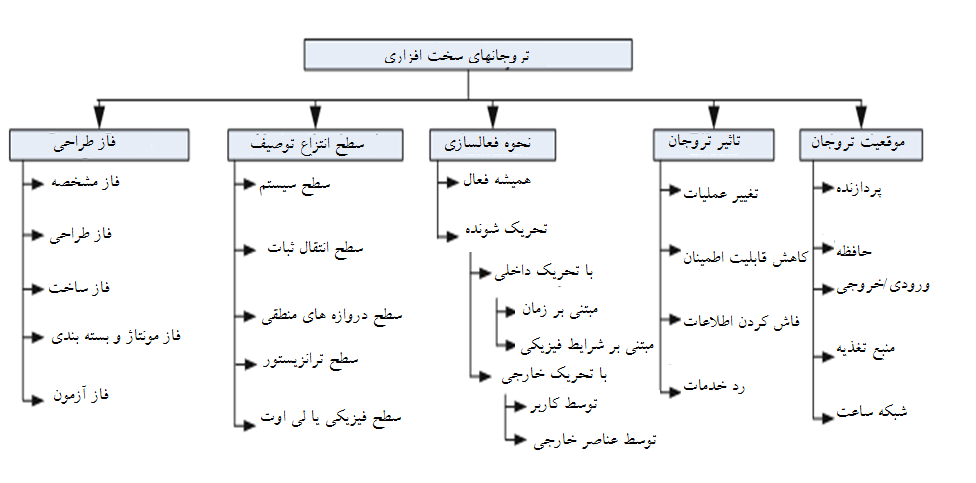
\includegraphics[scale=.7]{figs/fig1-2.png}
		\caption{دسته‌بندی ترواها}
		\label{figtax}
	\end{center}
\end{figure}


\section {مدل کردن تروا‌های سخت‌افزاری}
تروا‌های سخت‌افزاری از دو قسمت مدار تحریک و مدار بار   تشکیل شده‌اند. مدار تحریک درواقع شرایط فعال شدن تروا را نشان می‌دهد و مدار بار کاری را که تروا بعد از فعال شدن انجام می‌دهد، مشخص می‌کند. در زیر مدل‌های ساده شده و استانداردی از تروا‌های سخت‌افزاری را با مدارهای تحریک و بار متفاوت معرفی می‌کنیم.

\subsection {مدار تحریک}

مدار تحریک در تروا‌ها می‌تواند آنالوگ یا دیجیتال باشد. تروا‌هایی با تحریک دیجیتال می‌توانند توسط یک مدار ترکیبی یا یک مدار ترتیبی تحریک شوند.  در شکل  مدار تروای با تحریک دیجیتال ترکیبی نشان داده شده‌است. در این مدار اگر هر دو ورودی A,B همزمان صفر شوند، تروا فعال می‌شود و مدار XOR که به عنوان مدار بار استفاده شده‌است، در صورت فعال شدن تروا، باعث تولید نتیجه اشتباه می‌شود.

\begin{figure}
	\begin{center}
		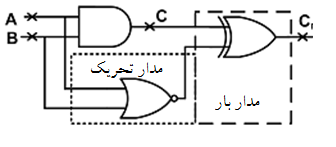
\includegraphics[scale=1]{figs/fig3-1.png}
		\caption[تروا با تحریک دیجیتال ترکیبی]
		{تروا با تحریک دیجیتال ترکیبی $\cite{chakraborty2009hardware}$}
		\label{fig3-1}
	\end{center}
\end{figure}

تروا‌های با تحریک ترتیبی که به آنها بمب ساعتی نیز می گویند، براثر رخداد رشته ای از وقایع یا براثر طولانی شدن یک رخداد خاص در مدت زمان از پیش تعریف شده، فعال می‌شوند. ساده ترین نوع مدار تحریک تروا‌های ترتیبی، شمارنده همگام است که بعد از رسیدن به یک تعداد شمارش، موجب تحریک تروا می‌شود. شکل \ref{fig2-3} یک نمونه از این دسته تروا‌ها را نشان می‌دهد.
\begin{figure}
	\begin{center}
		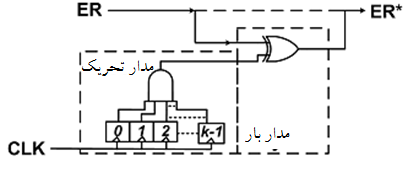
\includegraphics[scale=1]{figs/fig2-3.png}
		\caption[تروا با تحریک دیجیتال ترتیبی همگام]
		{تروا با تحریک دیجیتال ترتیبی همگام $\cite{chakraborty2009hardware}$}
		\label{fig2-3}
	\end{center}
\end{figure}

شمارنده‌های غیرهمگام نیز می‌توانند به عنوان مدار تحریک تروا‌ها استفاده شوند. نمونه ای از این تروا‌ها در شکل \ref{fig3-3} آمده است.
\begin{figure}
	\begin{center}
		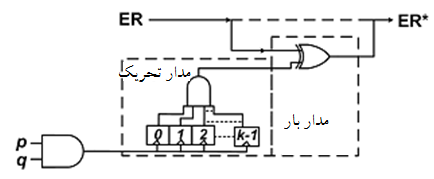
\includegraphics[scale=1]{figs/fig3-3.png}
		\caption[تروا با مدار تحریک دیجیتال ترتیبی از نوع شمارنده غیرهمگام]
		{تروا با مدار تحریک دیجیتال ترتیبی از نوع شمارنده غیرهمگام $\cite{chakraborty2009hardware}$}
		\label{fig3-3}
	\end{center}
\end{figure}

در این شمارنده‌ها، تعداد رخداد وقایع خاص، شمرده شده و بعد از رسیدن به یک مقدار از پیش تعیین شده، تروا تحریک می‌شود. مدار تحریک می‌تواند مشابه شکل \ref{fig4-3} ترکیبی از شمارنده‌های همگام و ناهمگام را شامل شود یا شامل ماشین‌ها‌‌ی حالت پیچیده با انواع و ابعاد مختلف باشد.
\begin{figure}
	\begin{center}
		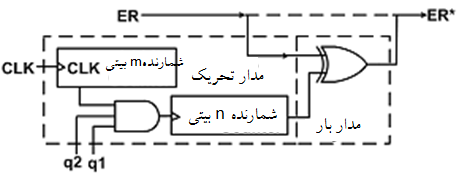
\includegraphics[scale=1]{figs/fig4-3.png}
		\caption[تروا با مدار تحریک دیجیتال ترتیبی با ترکیبی از شمارنده‌های همگام و ناهمگام ]
		{تروا با مدار تحریک دیجیتال ترتیبی با ترکیبی از شمارنده‌های همگام و ناهمگام $\cite{chakraborty2009hardware}$}
		\label{fig4-3}
	\end{center}
\end{figure}

تشخیص تروا‌هایی با مدار تحریک ترتیبی با استفاده از تولید بردارهای آزمون، به مراتب سخت‌تر از آنهایی است که از مدار تحریک ترکیبی استفاده می‌کنند. چراکه لازم است رشته ای از رخدادهای نادر را ایجاد کنیم تا تروا فعال شود.
دسته‌ای دیگر از تروا‌ها، آنهایی هستند که مکانیزم تحریکشان آنالوگ است. در این تروا‌ها، حسگرهای روی تراشه موجب تحریک تروا می‌شوند.  برای مثال در بعضی پژوهشها افزایش فعالیت مدار و در پی آن بالارفتن دمای تراشه به عنوان عامل تحریک تروا در نظر گرفته شده‌است $\cite{chen2008hardware}$.

\subsection {مدار بار}
تروا‌ها را می‌توان براساس مدار بارشان تقسیم‌بندی نمود. مدار بار می‌تواند آنالوگ یا دیجیتال باشد. تروا‌های دیجیتال می‌توانند مقادیر دیجیتال گره‌هایی از مدار را تغییر دهند یا محتویات بخشی از حافظه را دستکاری کنند. در مقابل، تروا‌های با مدار بار آنالوگ ، پارامترهای مدار مانند کارایی، توان مصرفی و حاشیه نویز را دستکاری می‌کنند. برای مثال در شکل  \ref{fig5-3} با اضافه کردن خازن بار، تاخیر مسیر تغییر داده شده‌است.
\begin{figure}
	\begin{center}
		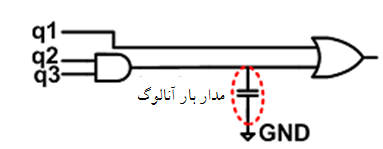
\includegraphics[scale=1]{figs/fig5-3.png}
		\caption[تروا با مدار بار از نوع آنالوگ ]
		{تروا با مدار بار از نوع آنالوگ $\cite{chakraborty2009hardware}$}
		\label{fig5-3}
	\end{center}
\end{figure} 
نوع دیگری از مدار بار آنالوگ، مداری است که موجب افزایش فعالیت سوئیچینگ شود تا بدین وسیله فرآیند کهولت مدار سرعت گیرد و زودتر از کاربیافتد. 
علاوه بر تروا‌هایی که گفته شد، بعضی تروا‌ها ممکن است حملات مبتنی بر نرم‌افزار را تسهیل کنند. از جمله حملات نرم‌افزاری می‌توان به تغییر سطح دسترسی، ایجاد درِ مخفی ورود به سیستم، و سرقت رمز عبور اشاره کرد.
